\fancychapter{Clustering Tweets with Self-Organizing Maps}

Tweets cathegorization with \ac{SOMs} requires a dataset to work on. Due to sistematic API restrictions, which where implemented in order to protect Twitter business model, gathering a dataset that directly maps to the social network is a great chalenge by itself. 
In order to cathegorize tweets with \ac{SOMs} first we used a dataset provided by INESC-ID. The dataset had almost 1TB of data in \ac{JSON} format.
Each tweet is comprised of multiple paramters. Figure~\ref{fig:json_tweet} shows how a tweet is represented in \ac{JSON} format. Inside the tweet there is also information about the user whom created the tweet, shown in Figure~\ref{fig:json_tweet_user} and enteties shown in Figure~\ref{fig:tweet_enteties}.
As can be seen in Figure~\ref{fig:json_tweet_user} no information about the social relations of the user which emited the tweet are present. Therefor in order to retrieve the social network in which a user is contained, it will be necessary to connect to the Twitter API. Crawling twitter is discussed in further depth in Chapter~\ref{chap:crawling_twitter}.  

\begin{figure}
  \begin{center}
    \begin{lstlisting}[language=json,firstnumber=1]
{ 
  "_id" : { "$oid" : "4fa14bc97e5617025fb14787" },
  "text" : "RT @FastCoDesign: A Paintbrush That Works On The iPad http://t.co/eWjEZAga (@sensubrushman)",
  "id_str" : "197701817864421376", 
  "coordinates" : null, 
  "in_reply_to_screen_name" : null, 
  "in_reply_to_user_id" : null,
  "possibly_sensitive" : false, 
  "favorited" : false, 
  "in_reply_to_status_id" : null, 
  "source" : "<a href=\"http://www.flipboard.com\" rel=\"nofollow\">Flipboard</a>", 
  "possibly_sensitive_editable" : true, 
  "contributors" : null, 
  "retweet_count" : 0, 
  "truncated" : false,
  "in_reply_to_status_id_str" : null,
  "geo" : null,
  "in_reply_to_user_id_str" : null,
  "entities" : { Enteties Object },
  "user" : { User object },
  "retweeted" : false,
  "id" : 197701817864421376,
  "place" : null,
  "created_at" : "Wed May 02 14:59:21 +0000 2012" }

    \end{lstlisting}
  \end{center}
  \caption{\ac{JSON} representation of a Tweet.}
  \label{fig:json_tweet}
\end{figure}



 \begin{figure}
  \centering
    \begin{lstlisting}[language=json,firstnumber=1]
 { "user_mentions" : 
   [{ "indices" : [ 3, 16 ], 
     "id_str" : "158865339",
     "name" : "Co.Design",
     "id" : 158865339,
     "screen_name" : "FastCoDesign" },
   { "indices" : [ 76, 90 ], 
     "id_str" : "534544812",
     "name" : "Matt",
     "id" : 534544812,
     "screen_name" : "sensubrushman" } ],
   "urls" :
     [ { "url" : "http://t.co/eWjEZAga",
         "indices" : [ 54, 74 ], "display_url" : "bit.ly/IAaKQf",
         "expanded_url" : "http://bit.ly/IAaKQf" } ],
   "hashtags" : [] }
    \end{lstlisting}
  \caption{Enteties mentioned inside the tweet}
  \label{fig:tweet_enteties}
\end{figure}

\begin{figure}
  \begin{center}
    \begin{lstlisting}[language=json,firstnumber=1]
    { "default_profile_image" : false,
      "friends_count" : 277,
      "profile_link_color" : "0084B4",
      "followers_count" : 105,
      "url" : null,
      "profile_image_url" : "http://a0.twimg.com/profile_images/690647919/19335_266330051104_635886104_3750428_5949465_n_normal.jpg",
      "id_str" : "26549290",
      "following" : null,
      "favourites_count" : 7,
      "notifications" : null,
      "profile_background_color" : "C0DEED",
      "statuses_count" : 331,
      "profile_background_tile" : false,
      "profile_background_image_url_https" : "https://si0.twimg.com/profile_background_images/79871480/DSC09031_2.jpg",
      "description" : "A Chicago-based designer and educator fascinated with the power of design to ignite change \r\n\r\n",
      "location" : "Chicago",
      "contributors_enabled" : false,
      "geo_enabled" : false,
      "time_zone" : "Central Time (US & Canada)",
      "profile_sidebar_fill_color" : "cde2e6",
      "listed_count" : 2,
      "profile_sidebar_border_color" : "C0DEED",
      "default_profile" : false,
      "show_all_inline_media" : false,
      "verified" : false,
      "protected" : false,
      "is_translator" : false,
      "profile_use_background_image" : true,
      "profile_image_url_https" : "https://si0.twimg.com/profile_images/690647919/19335_266330051104_635886104_3750428_5949465_n_normal.jpg",
      "name" : "Karma Dabaghi",
      "follow_request_sent" : null,
      "lang" : "en",
      "profile_text_color" : "333333",
      "id" : 26549290,
      "profile_background_image_url" : "http://a0.twimg.com/profile_background_images/79871480/DSC09031_2.jpg",
      "utc_offset" : -21600,
      "created_at" : "Wed Mar 25 17:55:26 +0000 2009",
    "screen_name" : "karmadabaghi"  }
    \end{lstlisting}
  \end{center}
  \caption{\ac{JSON} representation of a user, inside a tweet.}
  \label{fig:json_tweet_user}
\end{figure}


In order to better understand the dataset at hand, all the \ac{JSON} files where converted into \ac{CSV}in a way to reduce the size of the dataset. While tweets where being converted, \ac{URL} where removed due to the fact that most of them where minified in order to fit in less that 140 characters. Also, all tweets that where not identified as being in english where also removed. The tweet shown in \ac{JSON} format in Figure~\ref{fig:json_tweet} is converted to \ac{CSV} in Figure~\ref{fig:csv_tweet}.
%TODO find how many tweets have en user, and are not in english
%     count amount of different words with\without en filter and bloom filters
%     test whatlanguage to see if it is good to ientify language on tweets
%     size reduction
\begin{figure}
  \begin{center}
    \begin{lstlisting}[language=json,firstnumber=1]
    karmadabaghi,A Paintbrush That Works On The iPad @sensubrushman
    \end{lstlisting}
  \end{center}
  \caption{\ac{CSV} representation of a Tweet. The username is present in the first column and the tweet text on the last.}
  \label{fig:csv_tweet}
\end{figure}


Identifying tweets that where not in the english language was done through the usage of Ruby library called whatlanguage~\footnote{https://github.com/peterc/whatlanguage}, which tries to identify one language through Bloom Filters. Inside the tweet there is a field which identifies the user language, we found that x is not acurate. Removing tweets that weren't in the english language reduced the amount of different words in x and therefor will reduce the dimensional size of the \ac{SOM}.
The initial dataset features is described table x
 .
%\begin{tabular}{c | c}
  %Number of Files  & 337\\
  %Average File Size  & 337\\
%\end{tabulartabular}


Work done on the INESC twitter dataset with SOMs.
SOM implementations used, what where their strong points and weaknesses
SVM Dimension reduction and text treatment: compare multiple aproaches to reduce the svm size of tweets without losing relevant information

\fancychapter{Crawling Twitter for Social Relations}
\label{chap:crawling_twitter}
Explain the limitations of the INESC tweet dataset: crawlled by hashtag, social connections can only be obtained through connections to the twitter API, a lot of the tweets had no active users etc. 

\fancychapter{SOM Framework}
Explain what got me to create my own ruby library: everybody is making their own SOM algorithms ( ex.: websom, hsom etc ). Most implementations want to get as close to the metal as possible in order to deliver faster trainings, which makes the lybraries hard to modify. SOM framework is an modular implementation of the SOM algorithm in an higher level programing language which makes it easier to construct and test new SOM algorithms.

\fancychapter{Homophilic SOM}
Describe the alterations made to the default SOM algorithm in order to increase the homophilic (love of the same) relevance while cathegorizing socially connected data.

%% Sub multiple figures
%
%\begin{figure}[t]
%\centering
%\subfigure[caption for subfigure a]{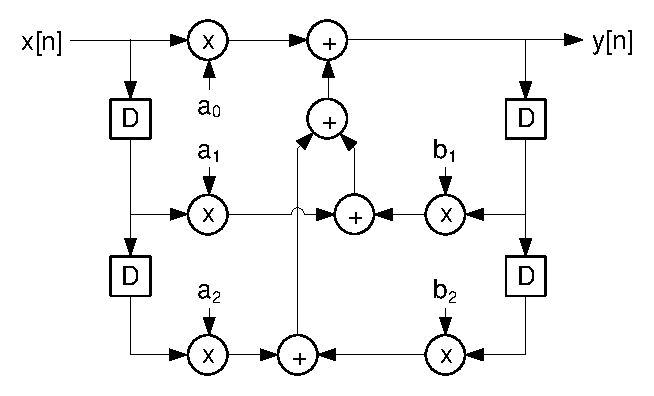
\includegraphics[scale=0.65]{images/img1.eps}\label{chp3:img1}}
%\hspace*{0.5cm}
%\subfigure[caption for subfigure b]{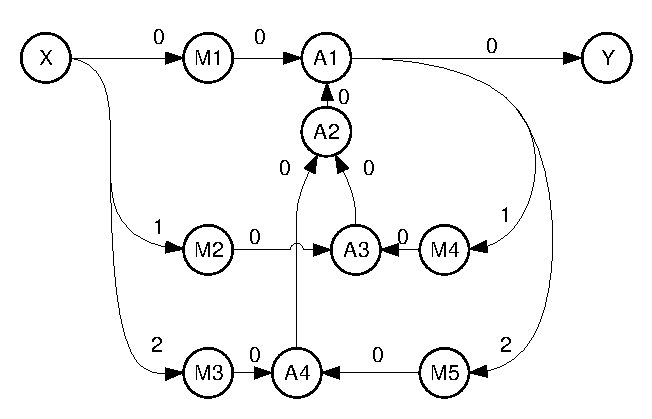
\includegraphics[scale=0.65]{images/img2.eps}\label{chp3:img2}}\\
%\caption{A figure example.}
%\label{fig:rmain figure}
%\end{figure}
%See the source code to see how to reference each of the subfigures \ref{chp3:img1} or \ref{chp3:img2}, or the main figure \ref{fig:rmain figure}.

%% how to add formulas
%There are several ways to define formulas (see the \textit{Short Math Guide for LaTeX} included in the package). The typical method is to use (see source code): 
%\begin{equation}
%a= b + c
%\end{equation}
%or
%\begin{align}
%c &= d \cdot e \nonumber\\
%d &= \mathbf{X}^{\mathsf{T}} \mathbf{Y}+ \gamma e^{2\pi}
%\label{chp3:eq1} 
%\end{align}
%or
%\begin{subequations}
%\begin{align}
%c &= d \cdot e \label{chp3:eq2:a} \\
%d &= \mathbf{X}^{\mathsf{T}} \mathbf{Y} + \gamma e^{2\pi}
%\label{chp3:eq2:b} 
%\end{align}
%\label{chp3:eq2} 
%\end{subequations}
%where $\mathbf{X}$ and $\mathbf{Y}$ are column vectors (you should always present the meaning of each parameter). The \textbf{AMS} packages allow to use the command \verb"\eqref" to cite equations such as \eqref{chp3:eq1},  \eqref{chp3:eq2:a},\eqref{chp3:eq2:b} or \eqref{chp3:eq2} (see source code).


% Ensure that the next chapter starts in a odd page
\cleardoublepage
 
